\documentclass{beamer}

\usepackage[utf8x]{inputenc}
\usepackage[T1]{fontenc}
\usepackage{ucs}
\usepackage[portuguese]{babel}
%\usepackage{nameref}
%\usepackage{makeidx}
\usepackage{bm}
\usepackage{color}
%\usepackage{epigraph}

%%using this way for tufte-book
%\usepackage{caption}
%\usepackage{subcaption} 
%\captionsetup{compatibility=false}
\usepackage{graphicx}

\usepackage{amssymb,amsmath, amsfonts, amsthm} 
\usepackage[final]{pdfpages}

%\usepackage[authoryear]{natbib}

\usepackage{keynote-vintage}

\input{confs/commands}

\begin{document}

    \title{Mecânica Estatística e \\Aprendizado Moral Social}%{{{
    \author{Jônatas Eduardo da Silva César}
    \date{\today}
    
    \begin{frame}
        \titlepage
    \end{frame}%}}}

    \begin{frame}{Moral}%{{{
       Correntes filosóficas
        \begin{itemize}
            \item Utilitaristas
            \item Deontológicas
            \item Virtudes Morais 
            \item ... 
        \end{itemize}
    \end{frame}%}}}
    
    \begin{frame}{Dimensões Morais}%{{{
        \begin{itemize}
            \item \textbf{Justiça / Trapaça}

            \item \textbf{Cuidado / Violência}

            \item \textbf{Lealdade (a grupos)/ Traição}

            \item \textbf{Respeito à autoridade / Subversão} 

            \item \textbf{Santidade / Degradação} 
       \end{itemize}
    \end{frame}%}}}

    \begin{frame}{Moral e ideologia política}%{{{
        \begin{figure} 
            \centering
            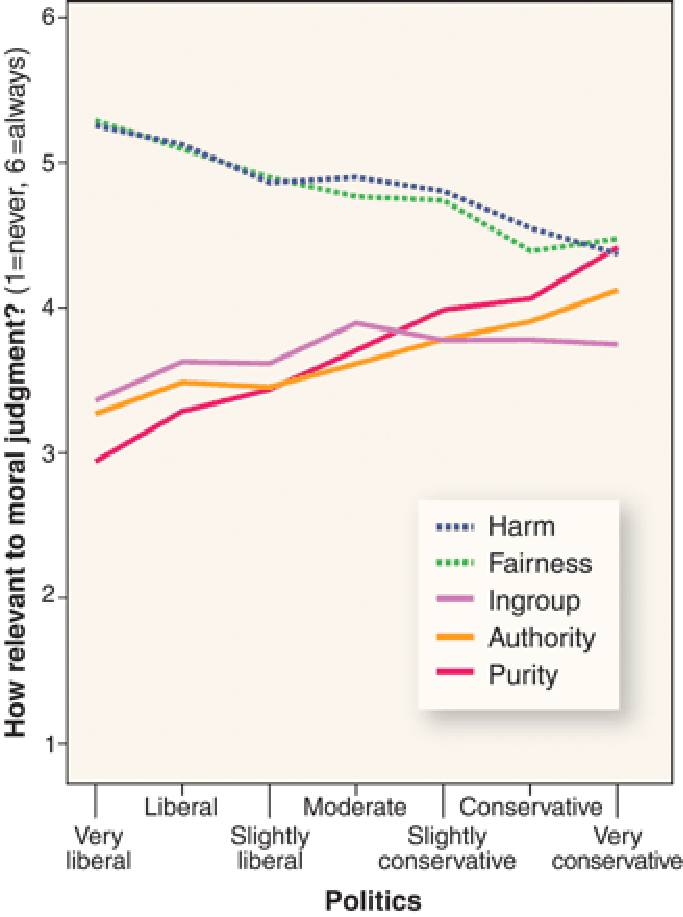
\includegraphics[scale=0.4]{Figures/haidt_science}
        \end{figure}  
        
    \end{frame}%}}}

    \begin{frame}{Aprendizado por reforço}%{{{
        \begin{figure}
        \begin{center}
        \includegraphics[scale=0.18]{Figures/dorsocial}
        \end{center}
        \end{figure}
    \end{frame}%}}}
    
    \begin{frame}{Go / No-GO}%{{{
    \begin{figure}
        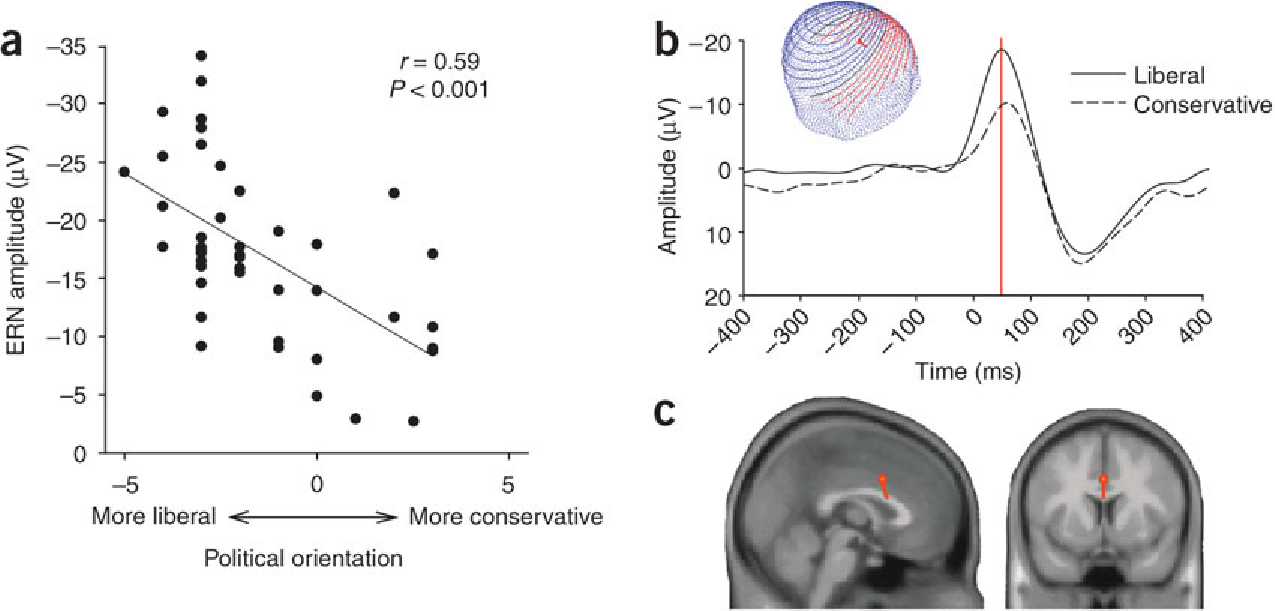
\includegraphics[scale=0.4]{Figures/amodio} 
        \end{figure}
    \end{frame} %}}}

    \begin{frame}{Complexidade e ideologia}%{{{
        \begin{figure}
            \centering
            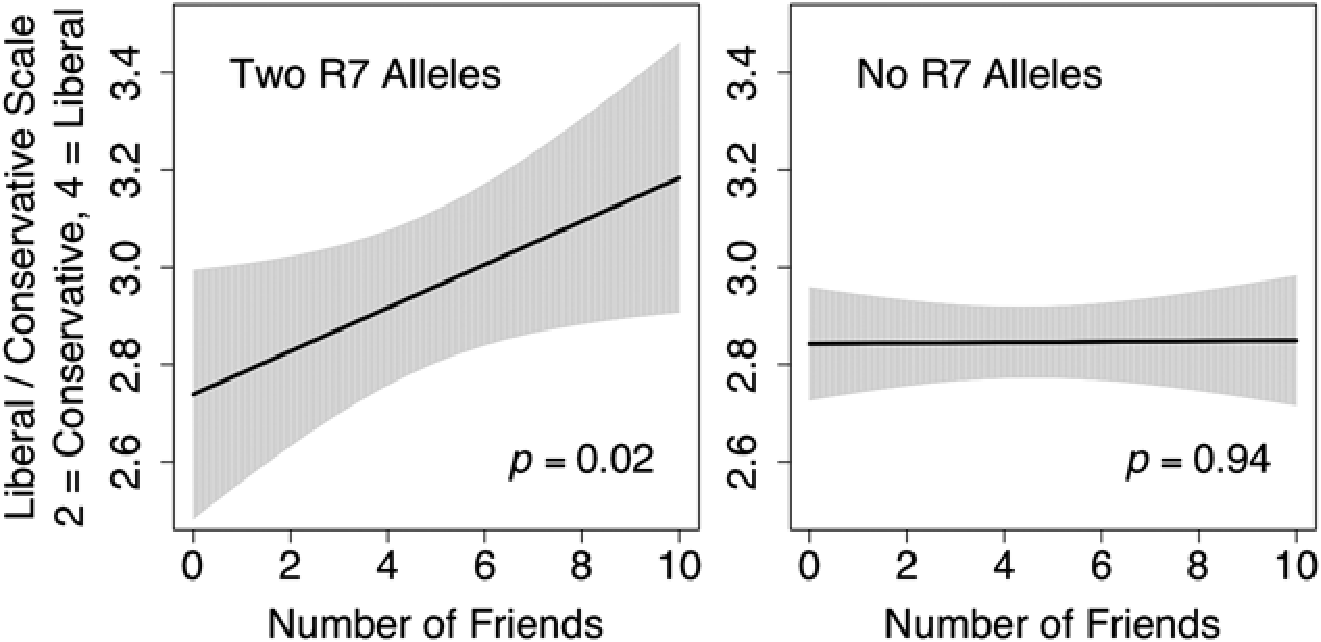
\includegraphics[scale=0.4]{Figures/DRD4_Fowler}
        \end{figure}
    \end{frame}%}}}

    \begin{frame}{Pressão Social}%{{{
        \begin{figure}
            \centering
            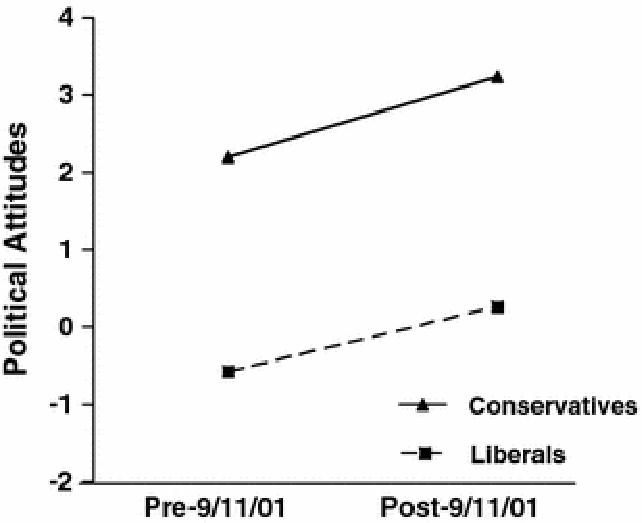
\includegraphics[scale=0.5]{Figures/nail_threat}
        \end{figure}
    \end{frame}%}}}

    \begin{frame}{Modelo}%{{{
       \begin{itemize}
           \item Matriz moral:\\
                 $\bm \omega_i = (\omega_{i 1},\ldots,\omega_{i 5})$

            \item Assuntos discutidos:\\
                $y_\mu=(\sigma_{j\mu},\bm x_\mu)$, onde \\
                $\sigma_{j\mu} =  sign(h_{j\mu})$,
                $h_{j\mu} = \bm \omega_j \cdot \bm x_\mu$

       \end{itemize}

    \end{frame}%}}}

    \begin{frame}{Fase 1}%{{{
        \begin{itemize}
            \item Equações do aprendizado
                \begin{align}
                    \ovl{\bm \omega}_i(t+1) 
                    &= \ovl{\bm \omega}_i(t) - 
                    \sigma_{j\mu} \bm x_\mu C_i(t)\pd{\mathcal E (t)}{z_\mu}; \nn
                    &= \ovl{\bm \omega}_i(t) + \sigma_{j\mu} \bm x_\mu  F(t); 
                    \label{eq:F1}\\
                    C_i(t+1) 
                    &= C_i(t) - C_i(t)^2 \pd{^2 \mathcal E (t)}{z_\mu^2}; \nn
                    &= C_i(t) + C_i(t) \pd{F(t)}{z_\mu}.
                    \label{eq:C}
                \end{align}
        \end{itemize}

   \end{frame}%}}}

   \begin{frame}{Função de Modulação}%{{{
       \begin{figure}
           \centering
           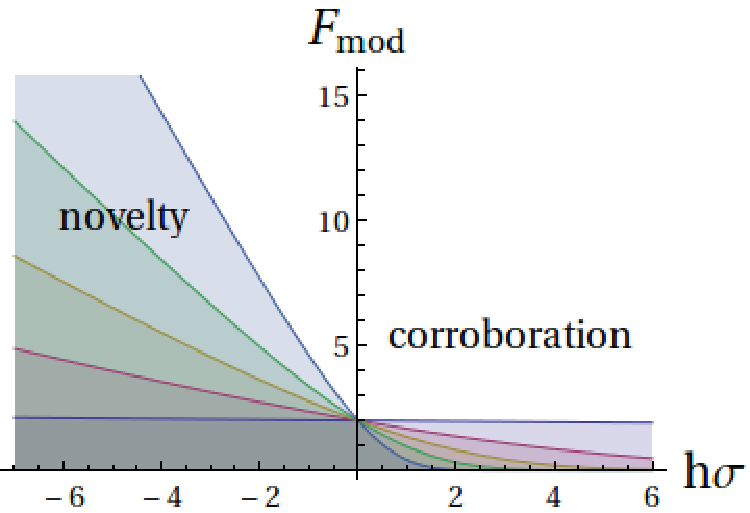
\includegraphics[scale=0.4]{Figures/funcmodruido0}
           \quad
           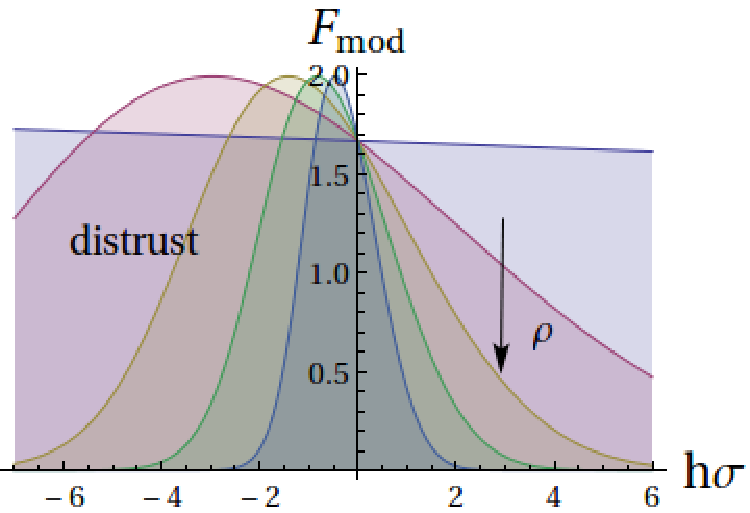
\includegraphics[scale=0.4]{Figures/funcmodruido02}
       \end{figure}

       \begin{align}
           F(z) = \frac{(1 - 2\epsilon)\exp\left(-\frac{z^2}{2C^2}\right)}
           {\epsilon + (1 - 2\epsilon)\Phi\left(\frac{z}{C}\right)}
           \qquad
           \rho_i(t) = \frac{1}{\sqrt{1 + C_i(t)^2}}
       \end{align}
   \end{frame}%}}}

   \begin{frame}{Fase 2}%{{{
    \centering
            \textit{Zeitgeist}:\\
               \[
               \mc Z \propto \frac{1}{P}\sum_{\bm x_\mu \in \mc X}\bm x_\mu.
               \]
            Dinâmica:\\
    \[
        \bm \omega_i \rightarrow \bm \omega_i' \text{ com prob. } 
        p = \min\{1,\exp( -\beta \Delta \mc E)\}
        \]
        onde
        \[
        \Delta \mc E 
        = \sum_{k\in\mc V_i } \mc E(h_i',\sigma_k) - \mc E(h_i,\sigma_k)
\]
   \end{frame}%}}}

   \begin{frame}{Parâmetros de Ordem}%{{{
       \begin{align}
           m = \mean{h_i}, \qquad 
           v = \mean{(h_i - \mean{h_i})^2};
       \end{align}
       
       \begin{figure} 
           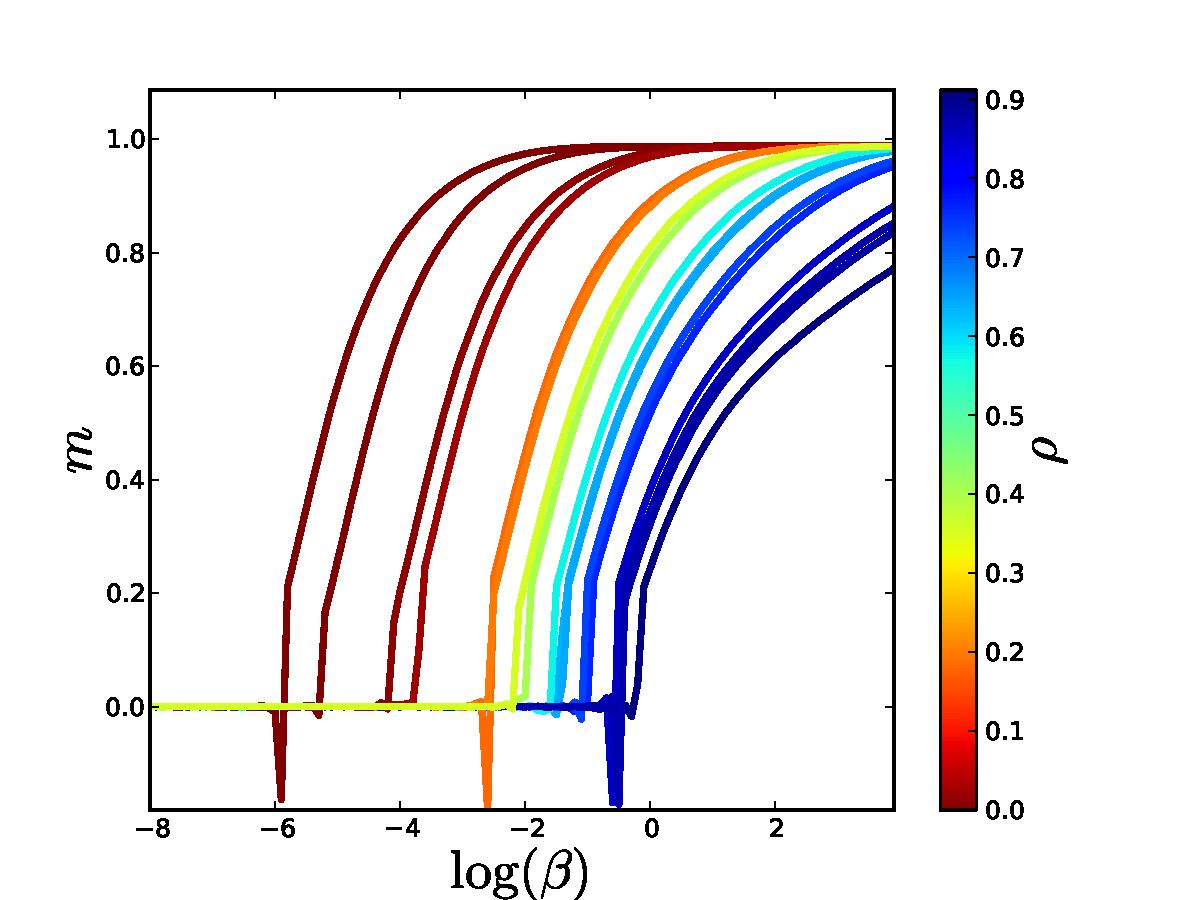
\includegraphics[width = 0.45\textwidth]{Figures/mag}
           \quad
           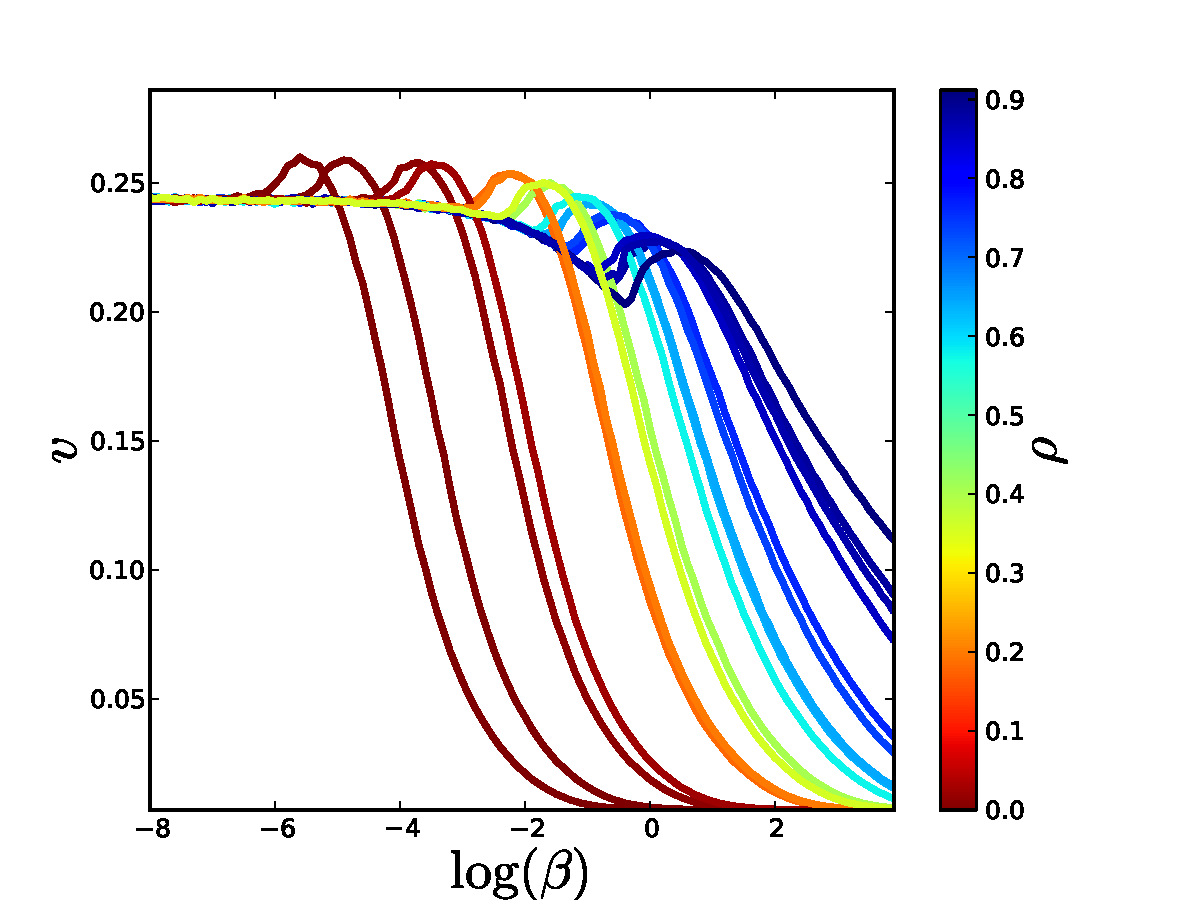
\includegraphics[width = 0.45\textwidth]{Figures/sigma}
       \end{figure}
   \end{frame}%}}}

   \begin{frame}{Transição de Fase}%{{{

       \begin{align}
           \chi = \beta\mean{(m - \mean{m})^2},
       \end{align}

       \begin{figure}
           \centering
           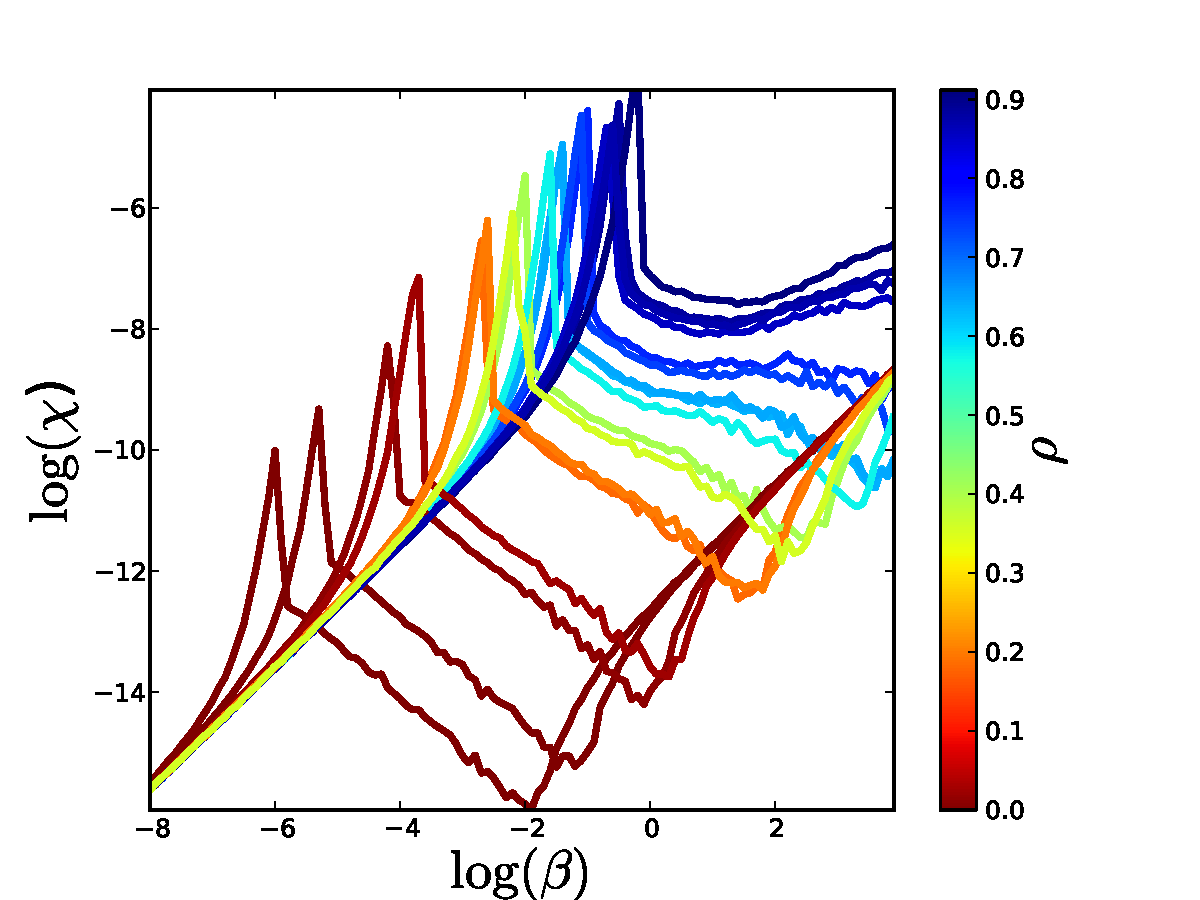
\includegraphics[width = 0.65\textwidth]{Figures/chi}
       \end{figure}
   \end{frame}%}}}

   \begin{frame}{Ideologia do Agente}%{{{

       \begin{figure}
           \centering
           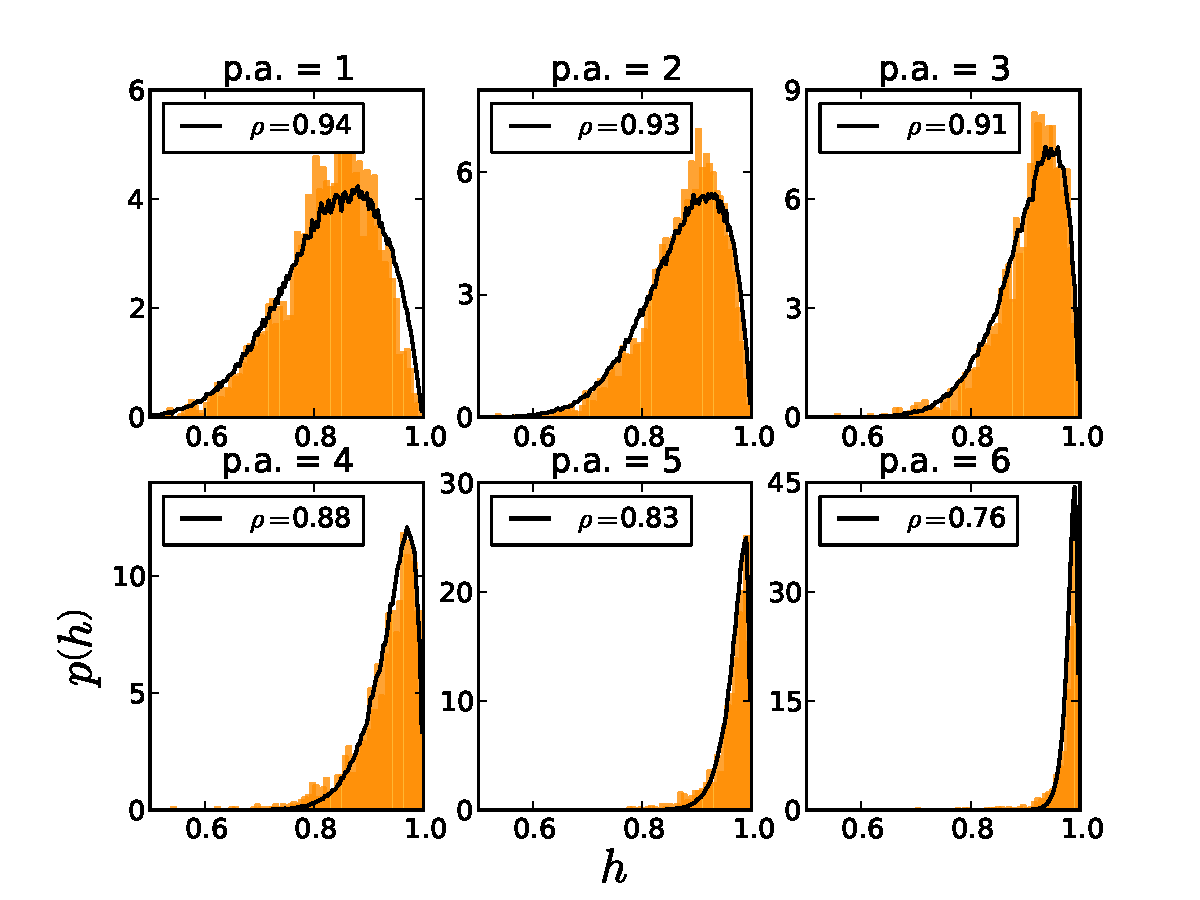
\includegraphics[scale=0.25]{Figures/hists_b38}
           \quad
           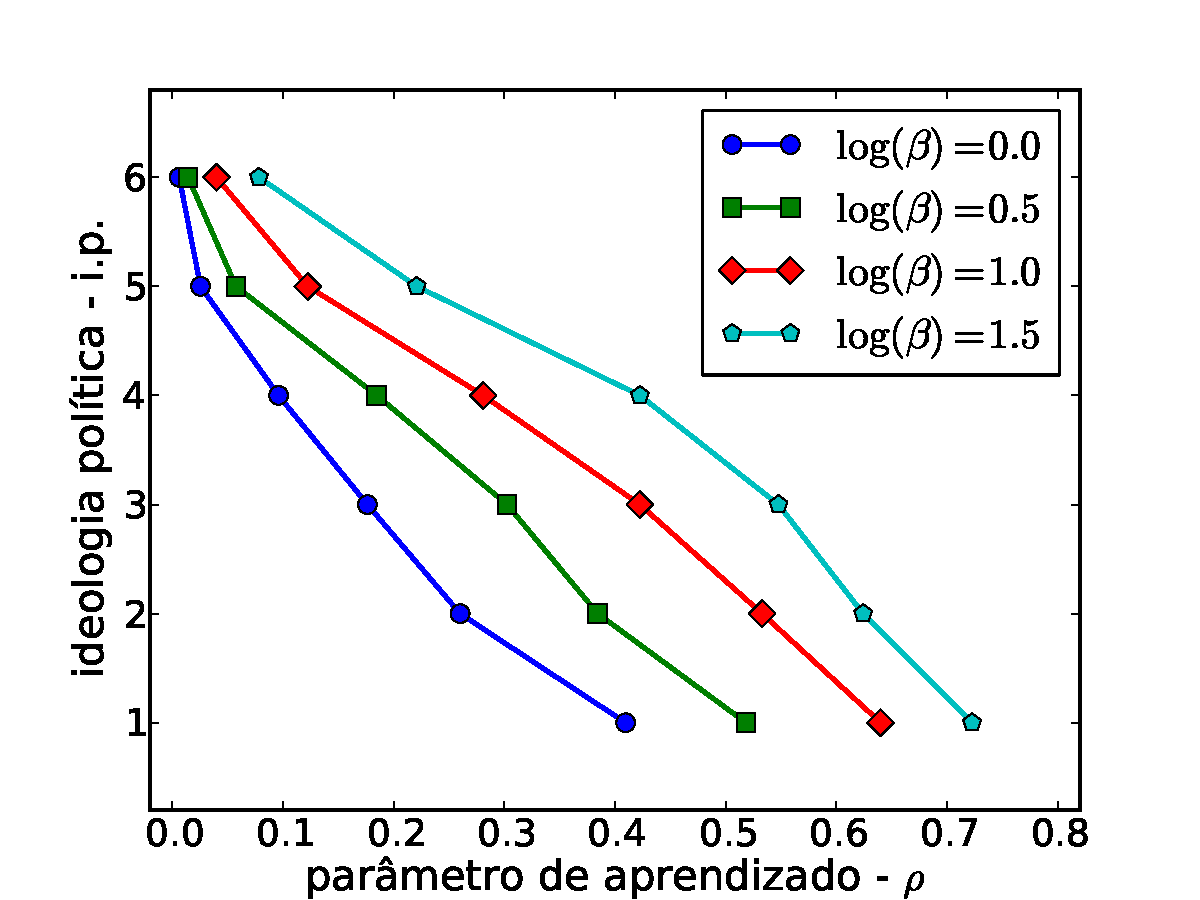
\includegraphics[scale=0.25]{Figures/pa-rho.pdf}
        \end{figure}
   \end{frame}%}}}

   \begin{frame}{Diagrama Político}%{{{
       \begin{figure}
           \centering
           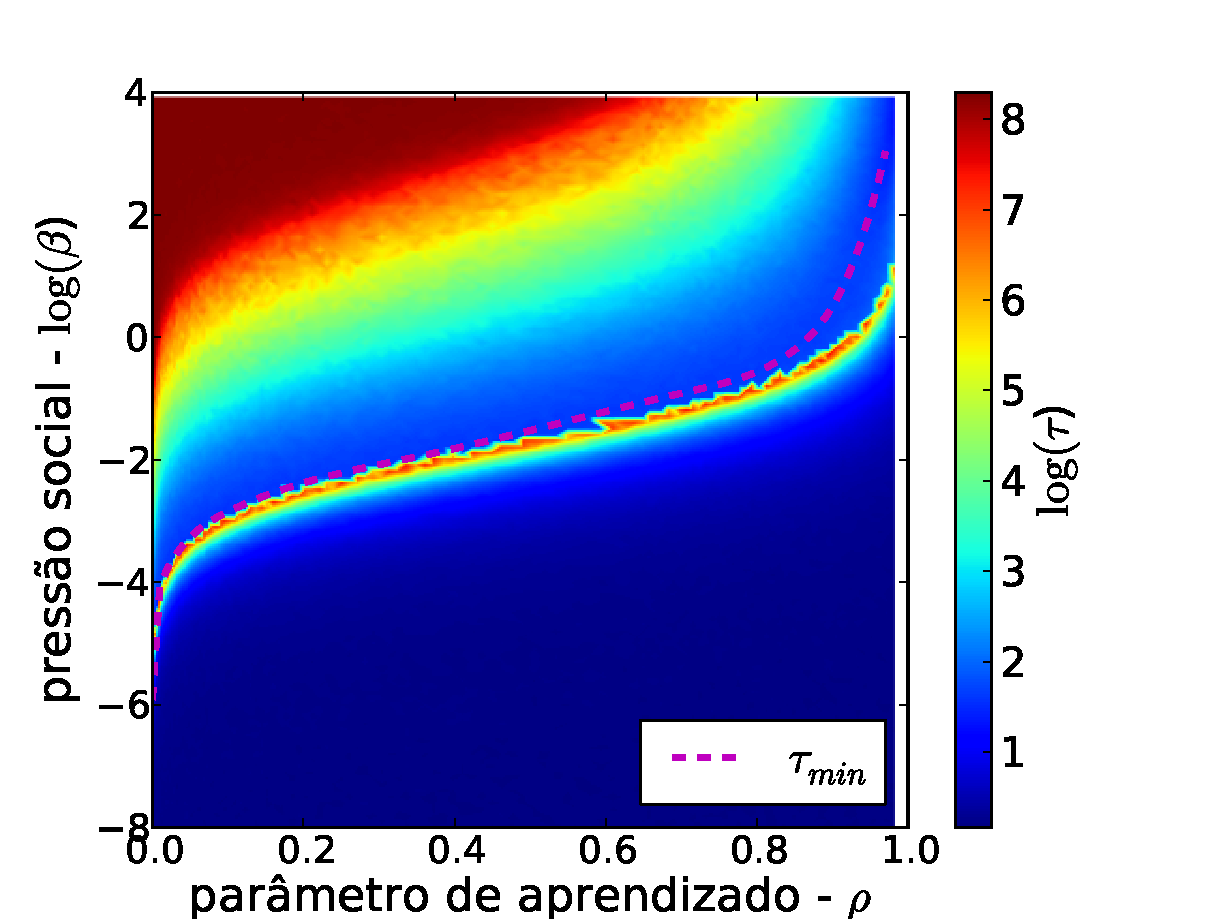
\includegraphics[scale=0.25]{Figures/tempocor_line.pdf}
           \quad
           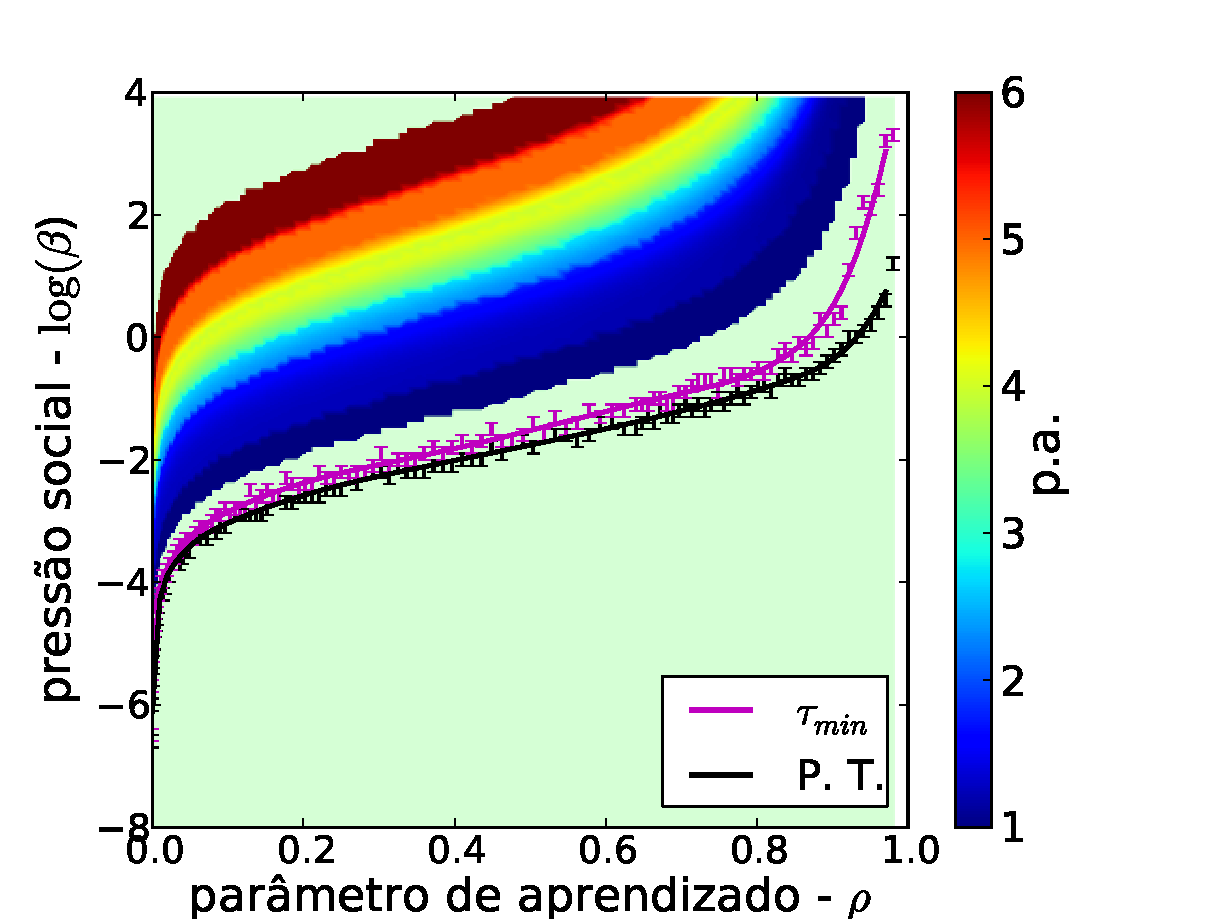
\includegraphics[scale=0.25]{Figures/padiag2.pdf}
       \end{figure}
   \end{frame}%}}}

   \begin{frame}{Ameaças e Conservadorismo}%{{{
       \begin{figure}
           \centering
           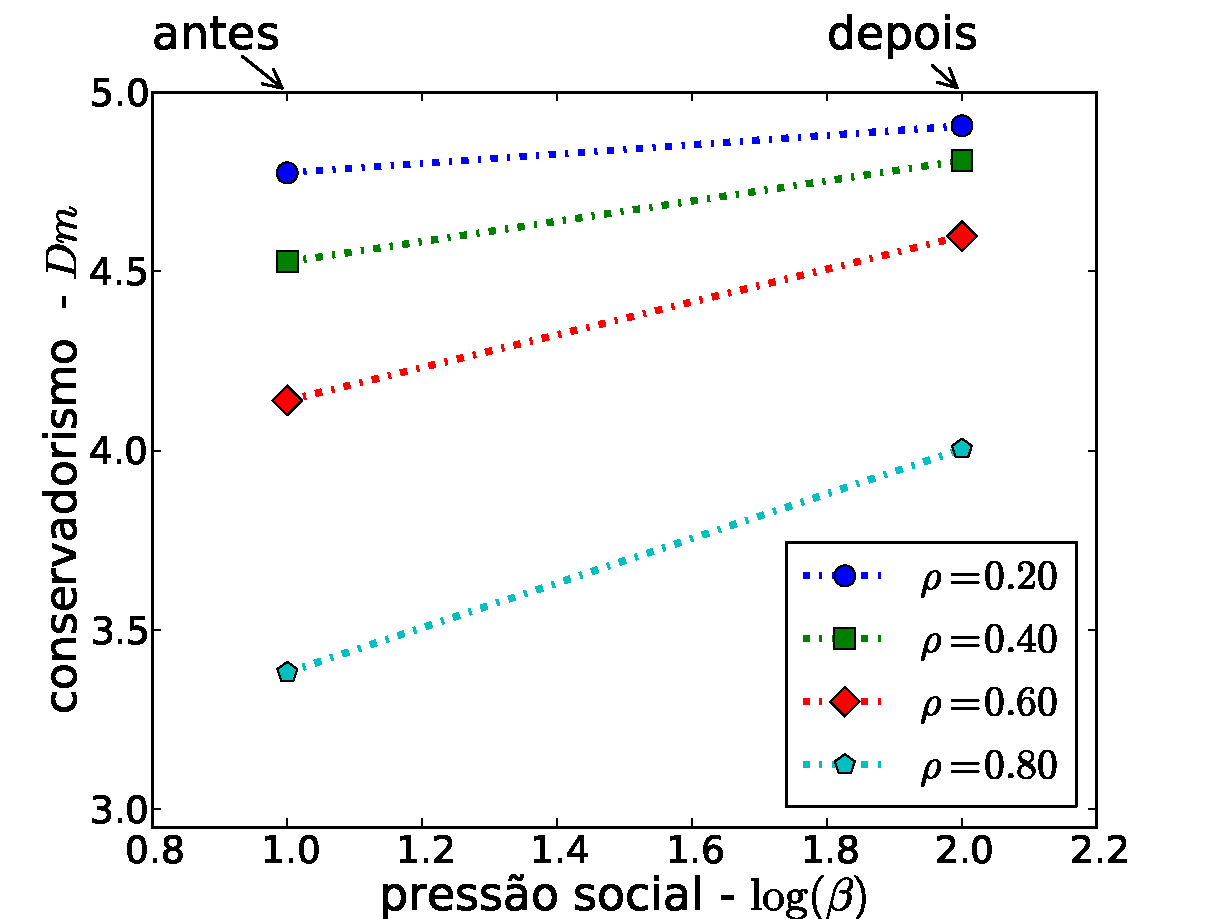
\includegraphics[scale=0.25]{Figures/threat.pdf}
           \quad
           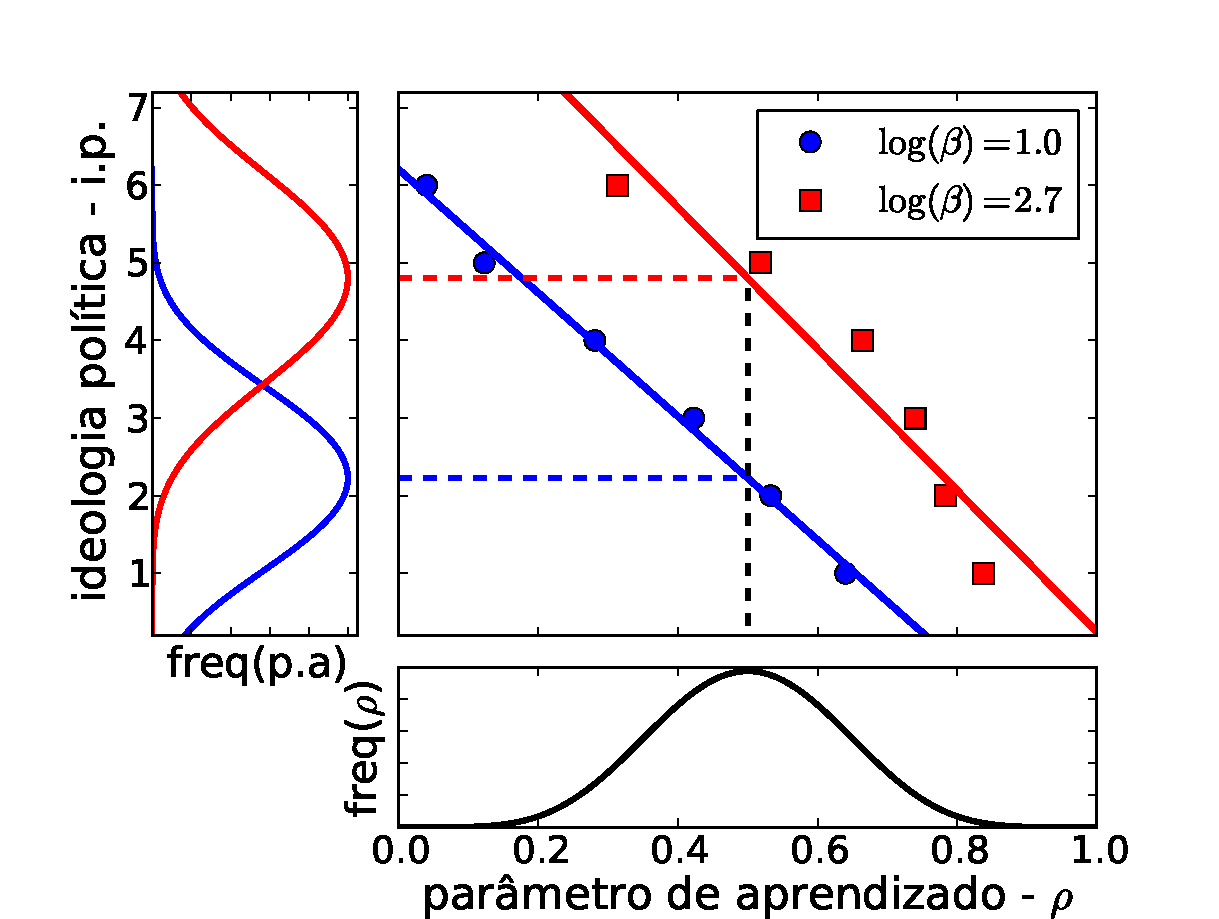
\includegraphics[scale=0.25]{Figures/dist-pa-rho.pdf}
       \end{figure}
   \end{frame}%}}}

   \begin{frame}{Conclusões}%{{{
       \begin{itemize}
           \item Liberalismo está positivamente correlacionado com quantidade de
               informação moral julgada nos anos de formação. 
           \item Agentes identificados como liberais apresentam menores tempos
               de adaptação para mudanças na sociedade.
           \item Aumento da pressão social favorece o conservadorismo.
       \end{itemize}

   \end{frame}%}}}


    %\bibliographystyle{plain}
    %\bibliography{Tese}
\end{document}
